\documentclass{article}
\usepackage[utf8]{inputenc}
\usepackage[margin=0.75in]{geometry}
\usepackage{booktabs}
\usepackage{listing}
\usepackage{amsmath}
\usepackage{algorithm}
\usepackage{array}
\usepackage{url}
\usepackage{cite}
\usepackage{complexity}
\usepackage{algpseudocode}
 \usepackage{graphicx}
 \usepackage{enumerate}
 \usepackage{subcaption}
 \usepackage[shortlabels]{enumitem}
 \renewcommand{\algorithmicrequire}{\textbf{Input:}}  % Use Input in the format of Algorithm  
 \renewcommand{\algorithmicensure}{\textbf{Output:}} % Use Output in the format of Algorithm  
 
 \begin{document}
 \begin{center}
   
     % MAKE SURE YOU TAKE OUT THE SQUARE BRACKETS
   
   \LARGE{\textbf{Enhanced Evolutionary Neural Architecture Search for Image Classification}} \\
       \vspace{1em}
       \Large{Project Proposal} \\
       \vspace{1em}
       \normalsize\textbf{ Bowen Zheng   }  
       \normalsize\textbf{ Shijie Chen   } 
       \normalsize\textbf{ Shuxin Wang  } 
       
       \vspace{1em}
       \normalsize{Advisor: Hisao Ishibuchi} \\
       \vspace{1em}
       \normalsize{Southern University of Science and Technology} 
 \end{center}
   \begin{normalsize}
   
     
     
   \section{Background \& Rationale}
       
     The great leap of computing resources in the past few decades made it possible to fully utilize the potential of neural networks. In recent years neural networks outperformed traditional methods in many fields of research, especially image classification. However, state-of-the-art architectures are carefully designed and tuned by researchers for a specific problem. Therefore, people start to think about automating the design of neural networks in the hope of finding the best-performing network architecture efficiently.

     Neural architecture search is a research field focusing on automating the design of neural networks. Currently, there are a few popular approaches, including reinforcement learning, Bayesian optimization, tree-based searching and genetic-based evolutionary algorithms. This project focuses on NAS for image classification problems. The reason is that this area is well explored and there exists many high-performance hand-crafted neural architectures as well as various NAS systems. Neural Networks targeting image classification are usually built upon basic components including convolution, polling, layer-wise normalization and activation layers. 
     
     Some datasets are widely used by the research community to compare performance. For example, the CIFAR-10 dataset and the larger CIFAR-100 dataset.
     % They provide good guidance and target for our project. In addition, neural networks for image classification are mostly built upon basic cells including convolution, pooling, normalization, and activation layers. This helps to shrink our search space.
     Our system built in the last project obtained a neural network with 76\% test accuracy on CIFAR-10. Through architecture modifications, we improved the performance of the initial network to 91.2\%. We expect to obtain a much more capable network through our enhanced ENAS system in this project.
   \section{Problem}
     Neural Architecture Search (NAS) refers to the process of automatically designing artificial neural network architectures\cite{elsken2018neural}. Research topics in NAS  includes search space, search strategy and performance estimation strategy. We have built an evolutionary NAS (ENAS) system which features a cell-based search space and an elite-parent preserving strategy. The ENAS system obtained a neural network with 76\% test accuracy on the CIFAR-10 dataset. 
     
     In this project, we enhance the ENAS system by (1) Validate the effectiveness of the elite-parent preserving population control policy; (2) Use a more promising initial network architecture; (3) Develop a neural network crossover operator; (4) Enhance local search capability of the system by differentiable architecture search as well as neural network approaches.
  
   \section{Objective}

   The objective of this project is to enhance the evolutionary neural architecture search algorithm that we built last semester. The specific objectives are as follows:
   \begin{enumerate}
     \item Validate the effectiveness of our novel elite-parent preserving population control policy.
     \item Develop a crossover operator based on network architectures.
     \item Improve the mutation operator by making use of network morphism.
     \item Improve neural network training with some training techniques. E.g. low fidelity, data augmentation and multi-GPU training.
     \item (Optional) Enhance local search ability via Differentiate Architecture Search \cite{liu2018darts} and RNN assisted search\cite{zoph2018learning}
   \end{enumerate}

   \section{Related Works}
   A lot of research works have been done in each of the three categories in NAS\@. Some proposed algorithms can design architectures that is on par of or even more capable than state-of-the-art hand-crafted networks.
   
   \subsection{Search Space}
   
   The search space of NAS determines the possible architectures a NAS algorithm can find.

   The simplest search space is the simple multiple-layer structure, in which a neural network $A$ is composed of multiple layers $L_i$ connected to the neighboring layers. In this case, the search space can be described by (1) The maximum number of layers (2) The type and dimension of each layer and their hyper-parameters\cite{chollet2017xception}\cite{baker2016designing}. 

   In more recent studies, some researchers use a cell-based search space in which possible architectures of cells are explored. A cell is nothing but a smaller neural network. The entire neural network is constructed by connecting several pre-defined cells. A cell has fewer layers but allows more complex architectures like skip connections between any layers\cite{cai2018path}\cite{real2018regularized}. The cell could be some hand-crafted neural networks that have already been proofed effective. The search space is therefore decreased to the possible arrangements of cells.

   In contrast to the above direction, some researchers also tried to search for effective cells and connect them at last in a predefined manner\cite{zoph2018learning}\cite{cai2018path}. The search space is greatly decreased in that each cell is comparably small. This method can also be easily transferred to other datasets\cite{zoph2018learning} since the structure of cells is not fixed.

   Recently, some researchers managed to optimize the overall architecture as well as the cells at the same time and obtained state-of-the-art result\cite{liu2019auto}.
   
   \subsection{Search Strategy}
   
   Many different search strategies can be applied to explore the search space discussed above. These methods include bayesian optimization, evolutionary methods, reinforcement learning and gradient-based methods. 

   Evolutionary algorithms have been used to evolve neural networks since 1989\cite{miller1989designing}. Earlier works use genetic algorithms to both optimize the structure of neural networks and train the networks\cite{stanley2002evolving}. However, with the birth of back-propagation (BP), recent works of neural-evolution use genetic algorithms only for optimizing neural architectures and use BP to train the networks\cite{real2017large}. In the context of NAS, the individuals in the genetic algorithm are neural network architectures and the genetic operations (crossover and mutation) are used to alter the architecture by adding/removing layers or changing the connectivity of nodes.

   Genetic algorithms show their diversity in how they sample parents, generate offspring and update population. Some work choose parents from a Pareto-optimal front\cite{elsken2018efficient} while others use tournament selection\cite{liu2018progressive}\cite{real2018regularized}\cite{real2017large}. When generating offsprings, some algorithms randomly initialize the weights of child networks. In comparison, Lamarckian inheritance is used in \cite{elsken2018efficient} so that child networks could inherit the weights of its parent and the training cost is reduced. To update population, some algorithms abandon least capable individuals\cite{real2017large} while some delete the oldest individuals\cite{real2018regularized}. A more sophisticated policy is developed by \cite{Hornby:2006:AAP:1143997.1144142} and \cite{DBLP:journals/corr/abs-1802-01548} in which the age of the individuals are taken into account.
   
   There are other methods that are used to implement NAS, including bayesian optimization, reinforcement learning, tree-based search and gradient-based methods. We don't discuss them here since we use evolutionary algorithms in our project.

   \subsection{Performance Estimation Strategy}
   One important issue in neural architecture search is the estimation of neural network performance. This is critical in the population update policy of evolutionary algorithms. 

   The simplest way to estimate performance is to train every searched network from scratch and test the desired performance metric, e.g. accuracy on the validation set. However, the training of neural networks is very time and computation consuming. 
    
   An alternative is to estimate performance on lower fidelities. More specifically, to train the network for a shorter period of time\cite{zoph2018learning} or on some subset of the dataset\cite{klein2016fast}. However, the estimate must ensure the result ranking of different networks must be the same as that of complete training. That is to say, there exists a trade-off between computational load and estimation fidelity.

   Another approach to estimate performance is based on learning curve extrapolation\cite{domhan2015speeding}. This method accelerates estimation by stop poor performance networks in the early stage of training based on statistical patterns of learning curves. Other researchers propose ways to predict neural network performance based on architectural and cell properties\cite{liu2018progressive}. 
   
   
   \subsection{Genetic Operators on Neural Networks}
   \subsubsection{Crossover Operator}
   The crossover operator is essential in evolutionary algorithms for its ability to improve the diversity of the population. It also produces offsprings that preserve good genes of their parents. However, designing a crossover operator for neural networks is very hard due to their chained structures and the difficulty of identifying the valuable part of a neural network structure. 
   We base our work on\cite{zhu2019eena} where multiple ways of neural network crossover are proposed. The basic idea is to obtain offsprings by combining components of parent networks. Considering the limits of model size, the author chose to let the offspring inherit the common structure (ancestor) of the two parents and randomly add the different parts.  
   \begin{figure}[H]
      \centering
      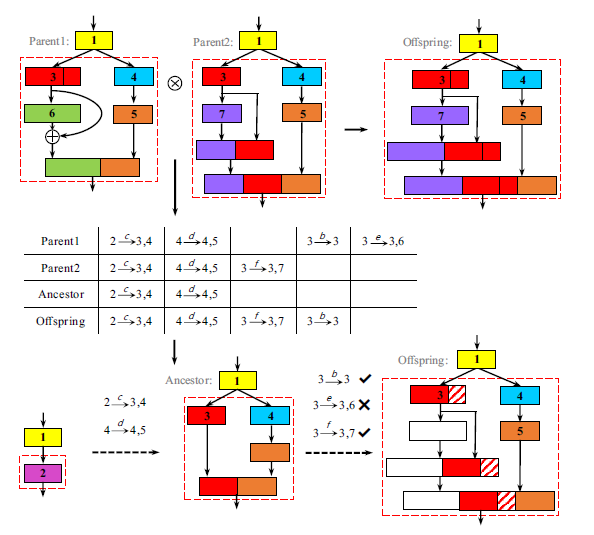
\includegraphics[width=0.6\textwidth]{figures/crossover.png}
    \caption{Illustration of neural network crossover operator\cite{zhu2019eena}. 1-7 represents different layers. b-f are mutation operators. Same colored boxes are the same layers.}
    \label{crsov}
   \end{figure}

   As is shown in Figure.\ref{crsov}, this cross over operator can combine the structure of the two parent networks. Experiments showed the effectiveness of this approach. Since we represent neural architectures as directed acyclic graphs (DAGs), such a crossover operator can be adopted.
   \subsubsection{Mutation Operator Based On Network Morphism}
   While crossover tends to explore a wider area of the search space, mutation operators perform small tweaks to approach the local optimal. Apart from the random mutation with heuristics mutation operator that was used in our last project, Network Morphism\cite{wei2016network} is another promising option for mutation operators.

   The focus of network morphism is to let the offspring architecture inherit the entire \textit{knowledge} of the parent network with the network function preserved. In \cite{wei2016network}, the author proposed a de-convolution based algorithm to fill parameters for width morphing, kernel size morphing and subnet morphing. Currently, network morphism makes the offspring network wider or deeper than its parent while being able to perform no worse than the parent network. 

   Due to the high computation load of network morphism and the difficulty in implementation, this is an experimental goal of this project.
   \begin{figure}[H]
      \centering
      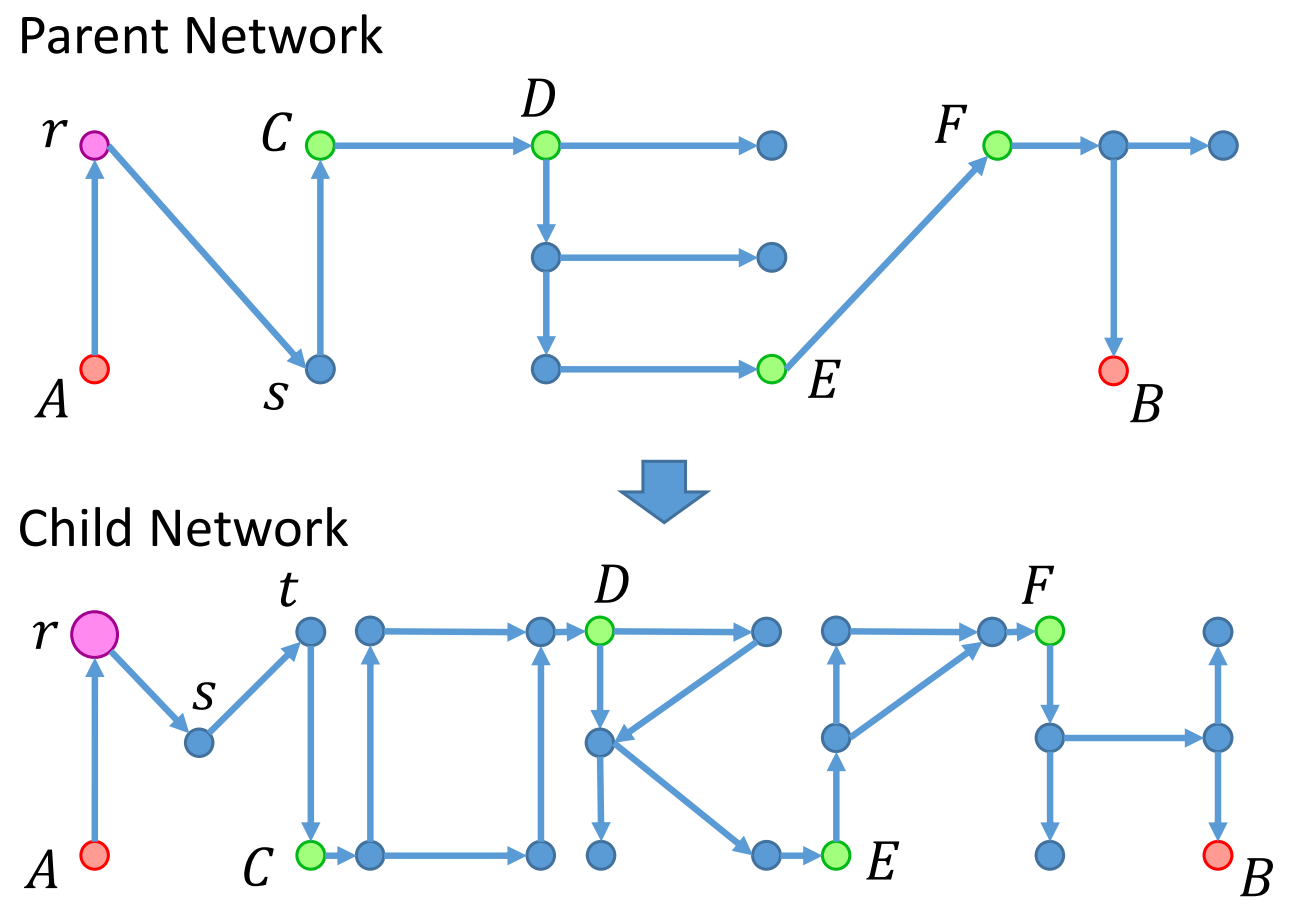
\includegraphics[width=0.6\textwidth]{figures/morph.png}
    \caption{Illustration of network morphism\cite{wei2016network}. Change of segment AC represents depth-morphing. The added layer \textit{t} involves width and kernel size morphing; Change of segment CD shows a subnet-morphing.}
    \label{morphing}
   \end{figure}

   \section{Methodology}
   We will enhance our work in the last semester by improving its search ability. A crossover mechanism will be designed based on \cite{zhu2019eena}. A mutation operator will be enhanced by network morphism \cite{wei2016network}. Our new search strategy should have a strong search ability on network structures.

   To test the effectiveness of our algorithm, we will experiment on image classification datasets including CIFAR-10, CIFAR-100.

   \section{System Design}
   This section describes the design of our ENAS system.
   \subsection{Cell-based Search Space}
 
   We explore a cell-based search space with 5 hidden cells, as is illustrated in Fig.\ref{f_artc}. Each edge in Fig.\ref{f_artc} represents a neural network unit. Each square represents a tensor in the neural network.
 
   \subsubsection{Neural Network Units}
   
   7 possible neural network units are suitable for image classification problems in our search space:
 
       \begin{enumerate}
         \item identity
         \item $3\times3$ average polling
         \item $3\times3$ max polling
         \item $1\times1$ convolution
         \item $3\times3$ depthwise-separable convolution
         \item $3\times3$ dilated convolution
         \item $3\times3$ convolution
       \end{enumerate}
 
   The search space is the possible connections between the states using different neural network units.
 
   \subsubsection{Cell Architecture Representation}
 
   We represent the architecture of a cell by a vector $R$ which is a vector of lists of tuple $R_{i} = \{(a_{i1}, b_{i1}), (a_{i2}, b_{i2}), ...\}$ where $a_i$ marks the input state of state $i$ and $b_i$ shows the unit used in the state transition connection.

   \begin{figure}[H]
     \centering
     \begin{minipage}[t]{0.45\linewidth}
       \centering
       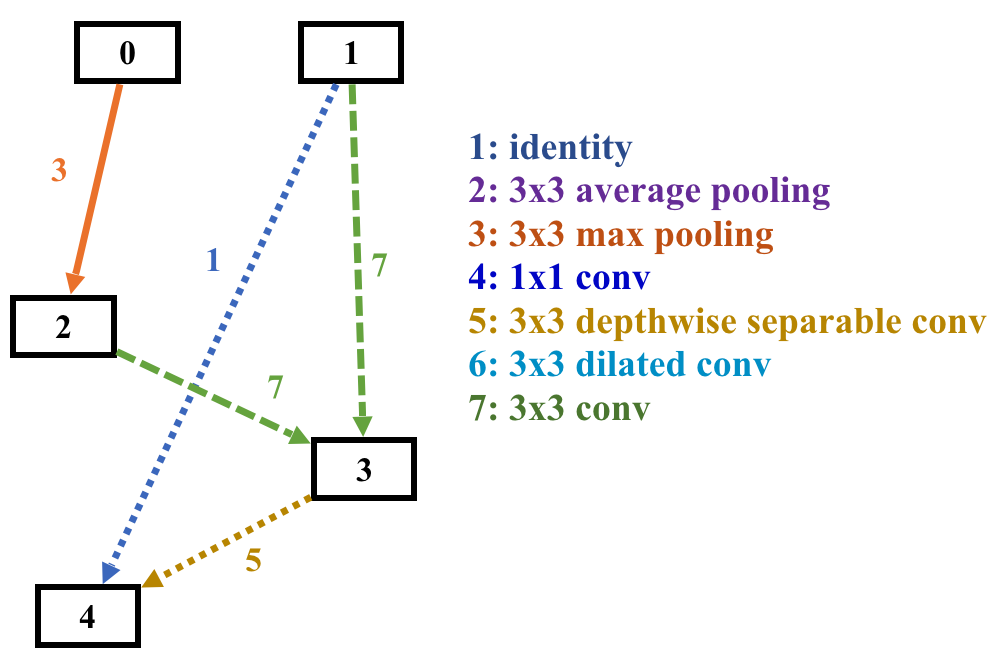
\includegraphics[width=0.9\textwidth]{figures/cellStruct.png}
    \caption{An example artitecture of a cell with representation $R=\{\{\}, \{\}, \{(0,3)\}, \{(2,7), (1,7)\}, \\ \{(1,1), (3,5)\}\}$.}\label{fig:digit}
    \label{f_artc}
     \end{minipage}
     \hfill
     \begin{minipage}[t]{0.5\linewidth}
       \centering
       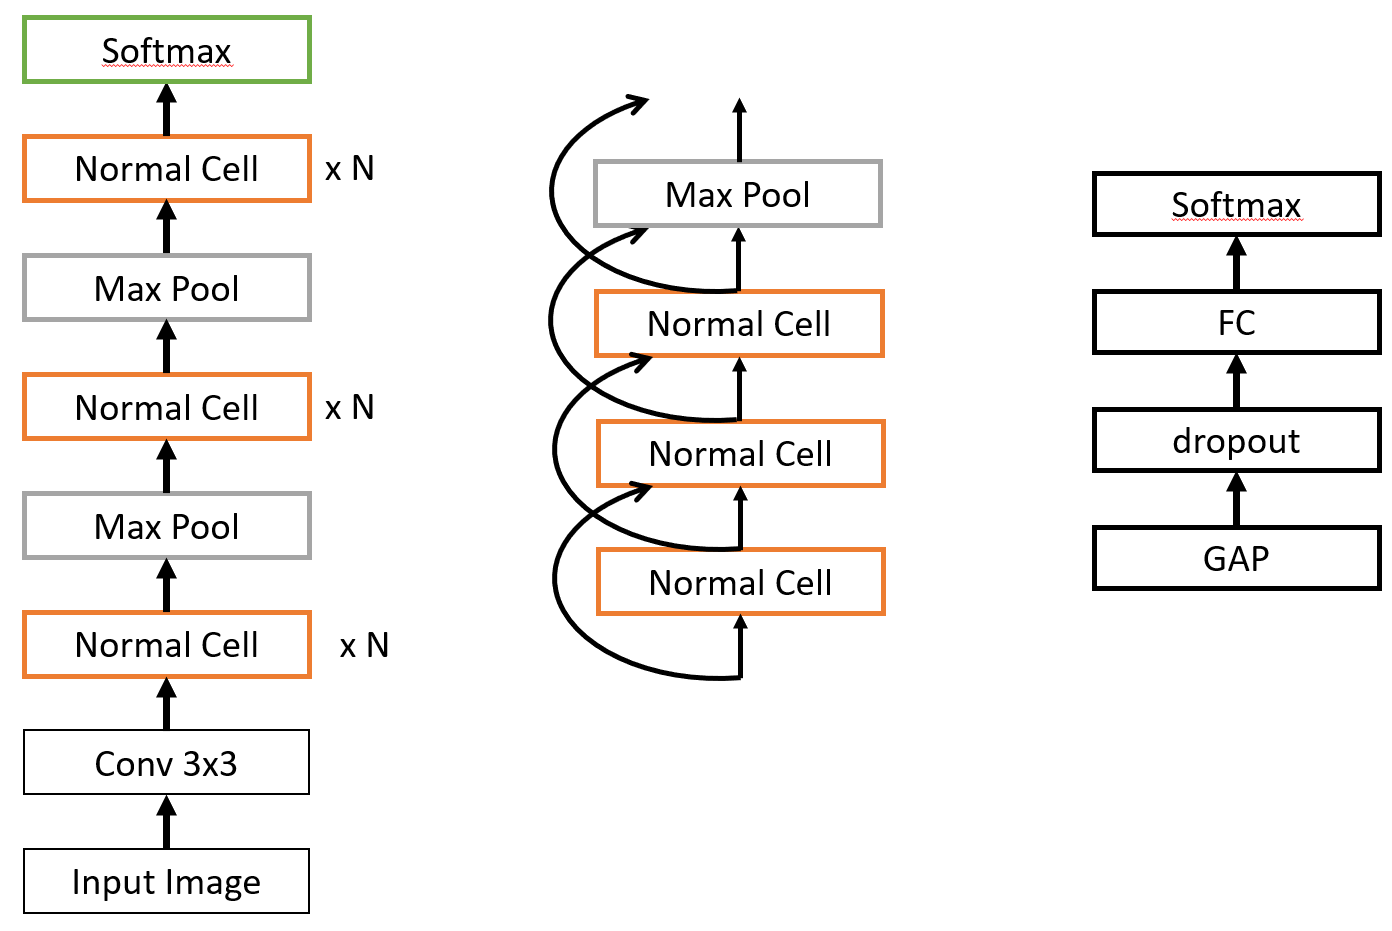
\includegraphics[width=0.9\textwidth]{figures/new_architecture.png}
    \caption{The simplified overall architecture of the total network. LEFT: outer structure. MIDDLE: detailed structure of normal cell stack. RIGHT: detailed structure of the Softmax unit.}\label{fig:digit}
    \label{total_artc}
     \end{minipage}
   \end{figure}


   \subsection{Overall Neural Network Architecture}
   As is illustrated in Fig.\ref{total_artc} overall network consists of input layer with 3x3 convolution, 6 ($N = 2$) identical cells, 2 polling layers, 1 global average polling(GAP) layer with dropout, 1 fully connected(FC) perceptron layers and 1 softmax layer. 
 
   For simplicity, all cells share the same structure. 

   Compared to the architecture of the ENAS system in the last project, we made the following changes:
   \begin{itemize}
     \item Intermediate nodes sum inputs instead of concatenating them.
     \item Skip connections are also used between cell stacks rather than within a single cell stack. We use factorized reduction for inputs with different sizes\cite{zoph2018learning} and 1x1 convolution for inputs with different numbers of channels to align dimensions.
     \item Add a 3x3 convolution layer after the input layer since complex network structures are more suitable for processing extracted features rather than raw inputs.
   \end{itemize}
   The initial solution generated under the new architecture reaches 91.2\% test accuracy on CIFAR-10.
   \subsection{Early Stop Performance Estimation}
 
   To accelerate the evolution process, we need to find a way to estimate the performance of a generated neural architecture. We use an early-stop strategy that trains the neural network with a small \emph{epoch} value. This approach can noticeably cut the training time of a network and at the same time provides a relatively reliable performance comparison metric.
 
   \subsection{Evolutionary Algorithm Framework}
   
   \begin{algorithm}[H]  
     \caption{ Elite Parent Preserving Evolution}
     \begin{algorithmic}[1]  
   
     \State $population\gets \phi$
     \State $entireGen\gets \phi$
     \State $generation\gets 0$
     
     \While{$population$ size$<N$}
     \State $newNetwork\gets networkInit()$
     \State $trainNetwork(newNetwork)$
     \State add $newNetwork$ to $popution$ and $entireGen$
     \EndWhile
     
   
     
     \While {$genetation < G$}
       \State $parent\gets$ select a parent from population using tournament selection 
       \State $child \gets mutate(parent)$
       \State $trainNetwork(child)$
       \State add $child$ to $popution$ and $entireGen$
       \If {accuracy of $child$ is better than $P\%$ individuals in population}
         \State extend the $lifetime$ of $parent$ by $t$
       \EndIf
       
       \ForAll {$individual$ in $population$}
         \State update the $age$ of $individual$
         \State remove current $individual$ if its $ age $ reaches its $lifetime$
       \EndFor
       
       
     \EndWhile
     
     
     \\  
     \Return the network model with highest accuracy in $entireGen$
  
   \end{algorithmic}  
   \end{algorithm}  
   For now, we follow the design of a cell based evolutionary NAS algorithm described in\cite{DBLP:journals/corr/abs-1802-01548} except that we propose a population update policy to preserve good parents. 
   Our evolutionary algorithm features an elite parent preserving strategy in which the lifetime of the parent whose child has a high accuracy rank within the total population is extended. In this way, we hope to preserve good genes in the population and produce more high-quality offsprings.
 
 The $population$ size is $N$ and the algorithm evolves $G$ generations in total. $entireGen$ stores all network models that we generated. $P$ and $t$ are hyper-parameters controlling the actual lifespan of an individual.
      
 In $networkInit()$, $N$ initial network models are generated. New Networks are generated in $Network Initialization$ with their $age $ being set to 1 and $lifetime$ set to the default value. The architecture of the network is obtained by randomly adding legal connections. A legal architecture is one with all hidden states having a positive in-degree and without any go-back connections. 
   
 \begin{figure}[H]
   \centering
   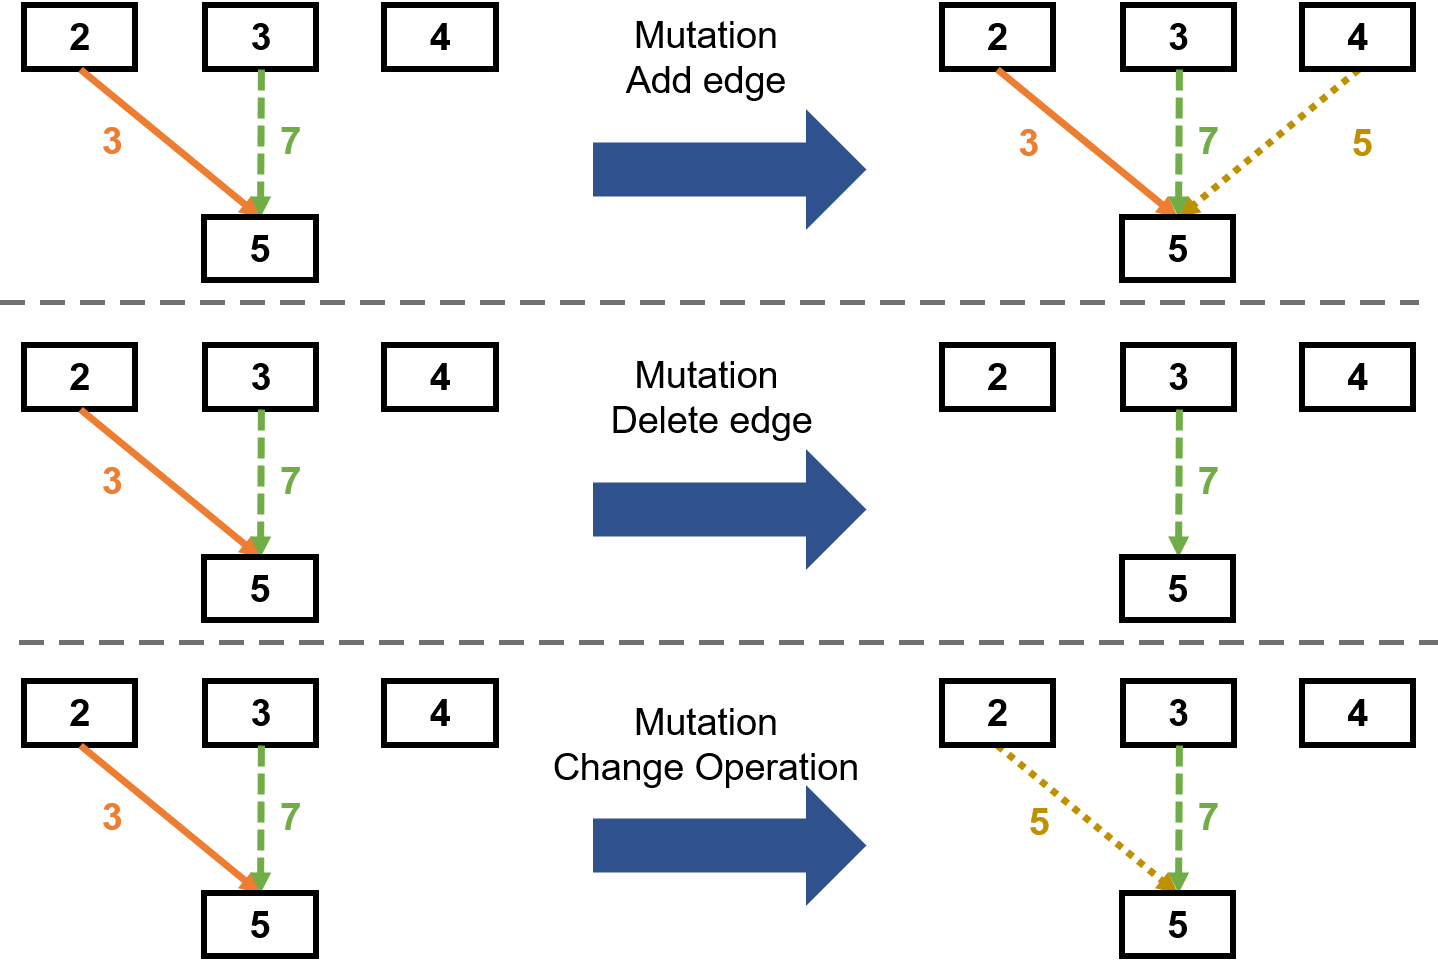
\includegraphics[width=0.45\textwidth]{figures/mutation.png}
   \caption{Three mutation operations.}\label{fig:digit}
   \label{mutation}
 \end{figure}
  \begin{algorithm}[H]  
     \caption{ Network Initialization}
     
     
     \begin{algorithmic}[1]  
         \Ensure A randomly generated network.
     \State $network\gets $ new $Network$
     \State $network.age\gets1$
     \State $network.life\gets $DEFALT\_LIFE 
     
     \State $arch\gets \phi$
 
     \ForAll  {$l$ in hidden layers } 
     \State $edge_l \gets \phi$
     \For {every input layers and hidden layers before $l'$}
     \If{$random<p$}
     \State $e \gets$ edge from $l'$ to $l$ with an randomly chosen neural network unit.
     \State $edge_l$.add($e$)
     \EndIf
         \EndFor
 
         \If{in-degree of $l>$0}
         \State  $e \gets$ legal edge to $l$ with a random unit.
         \State $edge_l$.add($e$)
         \EndIf
     \State $arch$.add($edge_l$)
         \EndFor
     
     \State $edge_{out} \gets \phi$
     \ForAll {$i$ with 0 out-degree}
       \State $e \gets$ edge from $i$ to output layer with identity unit.
       \State $edge_{out}$.add($e$)
     \EndFor
 
     \State $arch$.add($edge_{out}$)
     \State $network.arch=arch$
     \State $network.accuracy\gets getAcc()$
     \\
         \Return The $network$ generated.
         
     \end{algorithmic}  
 \end{algorithm}  
 
   When sampling the parent individuals, we randomly take $X$ individuals from the population and pick the one with the highest estimated accuracy. The mutation operation includes adding, deleting and altering an edge(NN unit). Fig.\ref{mutation} gives an example. At the same time, the resulting model must be valid and conform to our representation definition. Currently, mutation operations are stochastic. A better heuristic approach can be used to improve performance.
 
  \begin{algorithm}[H]  
     \caption{ Mutation Operation}
  
 
     \begin{algorithmic}[1]  
     \Require A network architecture $arch$
     \Ensure The $arch$ with a mutation
     
     
         \State Randomly pick a mutate position between two hidden layer.
         \While {$arch$ is unchanged or $arch$ is illegal}
         \State Apply mutation to the chosen position. 
     \EndWhile
     
     \State $edge_{out} \gets \phi$
     \ForAll {$i$ with 0 out-degree}
       \State $e \gets$ edge from $i$ to output layer with identity unit.
       \State $edge_{out}$.add($e$)
     \EndFor
 
     \State $arch$.replace($edge_{out}\_old$,$edge_{out}$)
 
     \\
     \Return arch
     \end{algorithmic}  
 \end{algorithm}  

 \section{Supplementary Experiments}
 In the last project, we proposed an elite-parent preserving strategy for population control in evolutionary algorithms. To identify the effectiveness of this strategy, we conducted a series of experiments on traditional optimization problems including binary string search and the traveling salesman problem (TSP). Then we compare our population control policy against the original population control policy with age\cite{zhu2019eena}. All results are averaged over 50 runs.

 \begin{figure}[H]
   \centering
   \begin{minipage}[t]{0.48\linewidth}
     \centering
     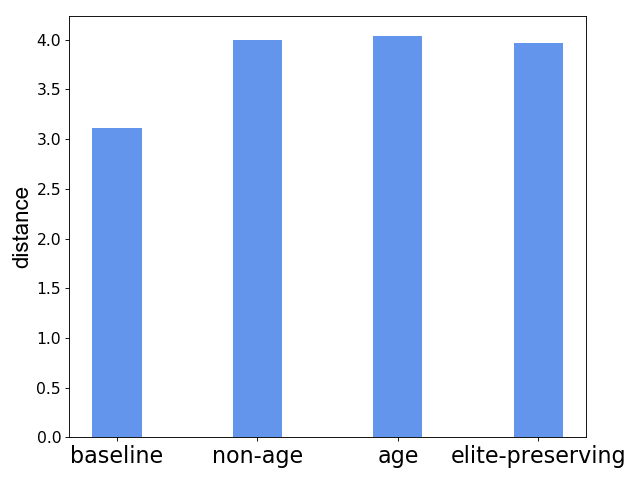
\includegraphics[width = 0.9\textwidth]{figures/tsp.png}
     \caption{Performance on TSP problem.}
   \end{minipage}
   \hfill
   \begin{minipage}[t]{0.48\linewidth}
     \centering
     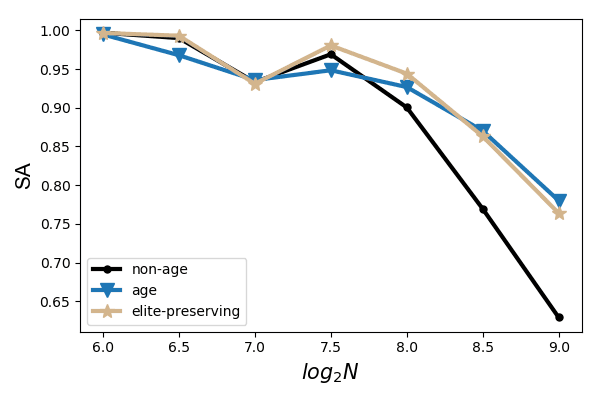
\includegraphics[width = 0.9\textwidth]{figures/01string.png}
     \caption{Performance on binary string search. SA is the simulated accuracy. $Log_2N$ denotes the length of the string.}
   \end{minipage}
 \end{figure}
\end{normalsize}

The TSP test problem is randomly generated with 20 cities. Population size is set to 500 and the evolutionary algorithms run 100,000 generations. The baseline score is obtained by an evolutionary algorithm in 250,000,000 generations.

We can see that our proposed elite-parent preserving population control strategy outperforms the original population control with age in \cite{zhu2019eena}. Both algorithms significantly outperform non-age evolution, especially when in a large search space.



\bibliographystyle{ieeetr}
% \bibliographystyle{plain}
\bibliography{ref}

\end{document}